%\op{Is it only validation? It seems that some of the paramters are also chosen based on these simulations. Also, the discussion seems to be using some parameters which are only made explicit later. For instance, in 7.1.2, the circuits with less than 1000 cells are described as useless for premium. The reson for that seems to only become clear when reading 8.3.1, which indicates that payments are made after 1000 cells. I wonder if, at the end of this section, and before the experimental analysis, it would make sense to add a frame that sums-up what protocol will be analyzed, including the parameters: what channels and circuits are created when, when is payment happening, when are channels closed, \dots}

\subsection{Data Collection}
\label{subsec:datacollection}

We deployed during two weeks a data collection system to look for empirical
temporal information about lifetime and bandwidth consumption in Tor circuits.
Our objective was to have a deeper understanding of typical Tor usage and
whether such usage can benefit from our channel-based payment system. For
example, these measurements might capture some notion about the type and
magnitude of potential premium traffic. We classify the traffic type based on
the service connection port. Besides the classical ports 80 and 443 used for web
traffic, we aggregate data from some other families including the WHOIS
protocol~\cite{daigle2004whois} and RWHOIS~\cite{williamson1994referral} from
ports 43 and 4321, respectively. The complete list of families is constructed
from the reduced exit policies which we run on our relays. This measurement
methodology allows us to reason based on application specific traffic.

% We interested to know about the distribution lifetime of Tor circuits for each
% port we allow. We are also interested to picture how many cells those circuits
% handled through their lifetime with some level of granularity.

\paragraph*{Efforts to preserve users privacy}

To ensure ethical experimentation, we first contacted the Tor research safety
board~\cite{torsafety}. The feedback we received was subsequently used to
refactor our data collection process (e.g., no metadata from any specific flow
or circuit should be written on disk).

Data from five old and very stable exit relays with a total bandwidth of 50
MiB/s was collected, stripped of origin metadata, and aggregated on a central
server. The data collected from each relay is itself an aggregation which we
perform inside the relay's memory. The aggregation is done only for ``active
circuits'' from the exit relay perspective. We consider a circuit active when it
has received a connection request to an IP address on the internet.
%The data collection is probabilistic; only 30\% of the circuits processed by our
%relays were considered in order to maintain plausible deniability on the
%clients' behalf.
The aggregation is done inside bins of configurable size for every different
traffic family we consider. Once we collected enough data from a single family
(1600 circuits of a same family), we dump the aggregated information on the
disk, clear the relay memory, and resume a new session. The final information
obtained contains sessions of aggregation of 1600 circuits over an unspecified
time frame that is implicitly determined by the rate of user activity. The
following data was considered:

\begin{itemize}
\item \textbf{Time Profile}: The number of cells in each time interval
  (configured to be 5 seconds) since the success of the DNS request. This
  information sums inbound and outbound cells, and is aggregated over circuits
  by addition.
\item \textbf{Total Counts}: The total amount of cells processed by a circuit.
  This information is aggregated by taking the mean of fixed-size nearest
  neighbor bins.
\end{itemize}

Crucially, we do not record information linked to any single particular user
flow on disk.
%The code used for the data collection will be made available for
%audit online.

\paragraph*{Observations}

\begin{figure*}[t] \centering
\begin{subfigure}[t]{0.47\textwidth} \centering\centering
  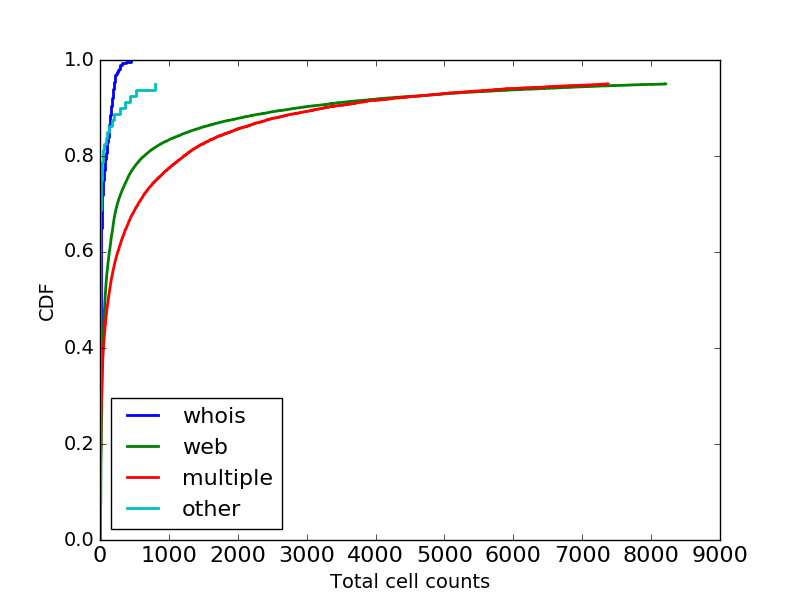
\includegraphics[width=0.7\textwidth]{images/totcellcountscdf.png}
  \caption{Total Counts --- Distribution of circuit size with respect to the
    total number of cells processed}
\label{fig:statsb}
\end{subfigure}
\begin{subfigure}[t]{0.47\textwidth} \centering
  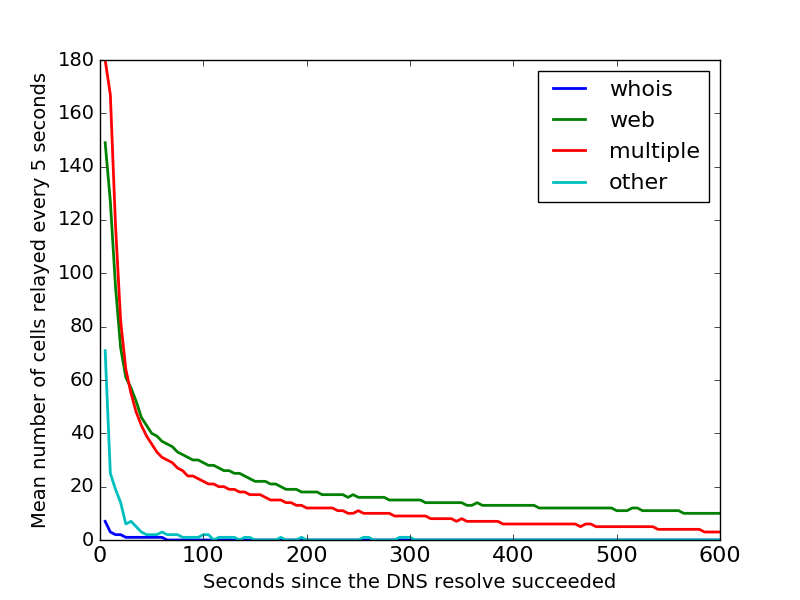
\includegraphics[width=0.7\textwidth]{images/exitmeasurement.png}
  \caption{Time Profile --- Average distribution of traffic across circuit
    lifetime beginning with the first DNS request.}
  \label{fig:statsa}
\end{subfigure}
\caption{Data collection from 5 old and stable exit relays with a cumulative
  bandwidth of $\approx$50 MiB/s}
\label{fig:stats}
\end{figure*}


Our measurements successfully captured several important pieces of information
for the design and justification of moneTor. For example, one important task is
to determine the number of potential users that could benefit from paid traffic.
From Figure~\ref{fig:statsb}, we observe that $\approx 82\%$ of circuits
carrying only web traffic exchanged less than 1000 cells. While we cannot deduce
any statements about users, we can speak to the fraction of circuits that may
benefit from a payment channel in the Tor network, since around $50\%$ of them
do not carry data and less than $17\%$ of them carry at least one web page. The
remaining $18\%$ would appear to be better candidates for moneTor.

It is also evident from Figure~\ref{fig:statsa} that most of the traffic is
usually carried within the first few tens of seconds, and that all types of
traffic we collected seems to follow the same rule. From that result, we believe
that the reliability of payment is critical within the first few seconds,
especially from a relay viewpoint. This result highlight our choice to extend
Bolt to offer high fairness. Our payment channels should ideally be established
and ready before the user begins to use the circuit. While this result cannot be
guaranteed for an unbounded number of circuits, a well-designed preemptive
circuit build strategy should do a sufficient job of eliminating channel
setup/establish latency in the average case.

%% In another area of research, it may be interesting to point out that since %
%$\approx 50\%$ of users do not carry data after their DNS request, some %
%adversary doing end-to-end correlation may prefer to use active attacks over %
%passive correlation to capture more identities.

\section{Experimental Validation}
\label{sec:experimentations}

Having established the empirical context for a channel payment scheme, we
validated our technical design via experiments performed on a prototype software
implementation within the native Tor codebase.

\subsection{Prototype}

\begin{figure*}[t] \centering
	\begin{subfigure}[t]{0.32\textwidth} \centering
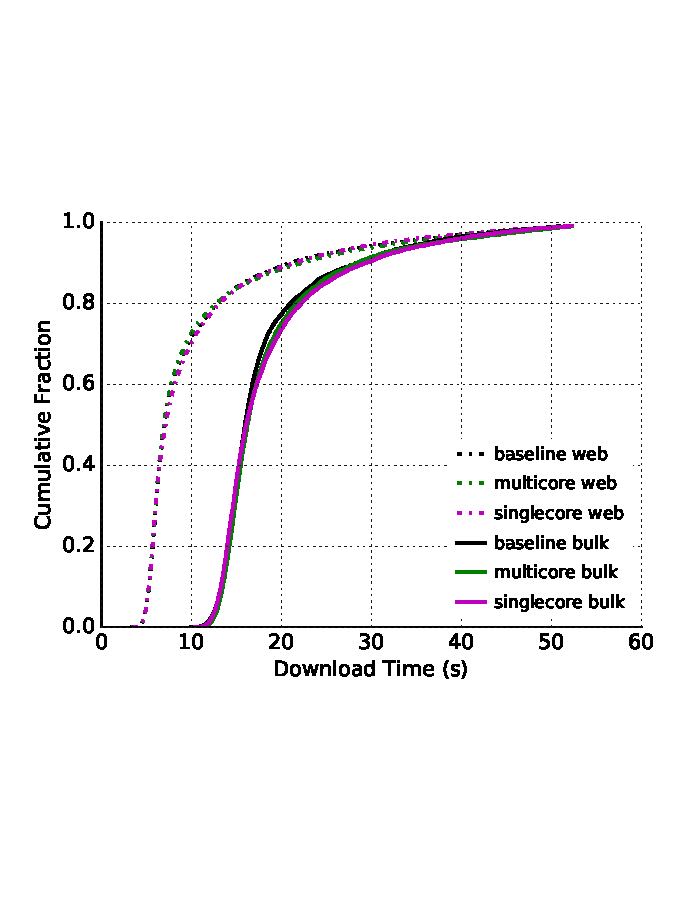
\includegraphics[clip, width=1.0\textwidth]{images/overhead_downloadtime.pdf}
		\caption{Download Time Overhead - Web + Bulk}
		\label{fig:overhead_ttlastbyte}
	\end{subfigure}
	\begin{subfigure}[t]{0.32\textwidth} \centering
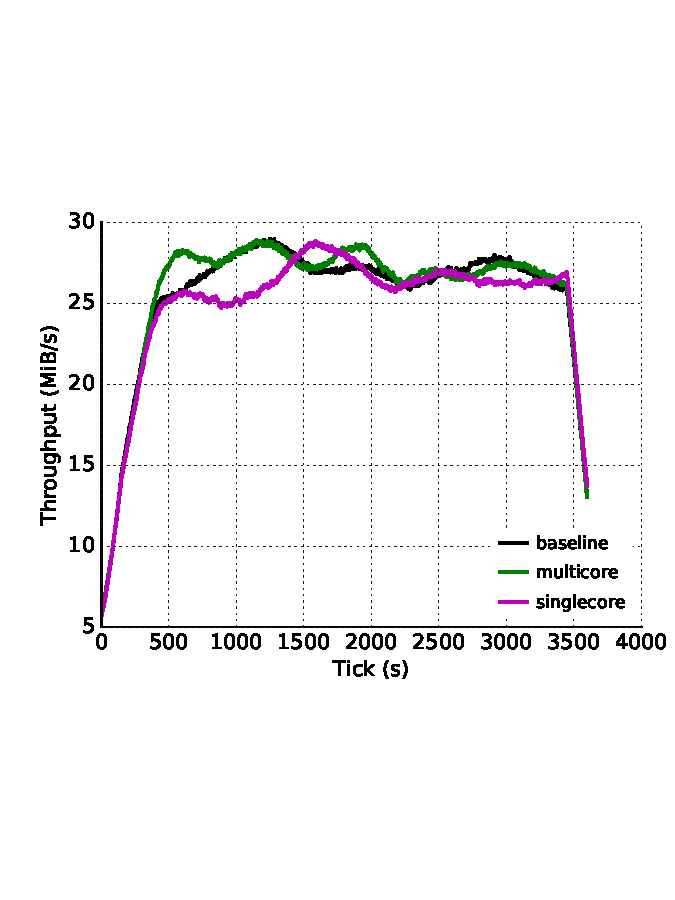
\includegraphics[clip, width=1.0\textwidth]{images/overhead_throughput.pdf}
		\caption{Throughput - Compared to baseline}
		\label{fig:overhead_throughput}
	\end{subfigure}
	\begin{subfigure}[t]{0.32\textwidth} \centering
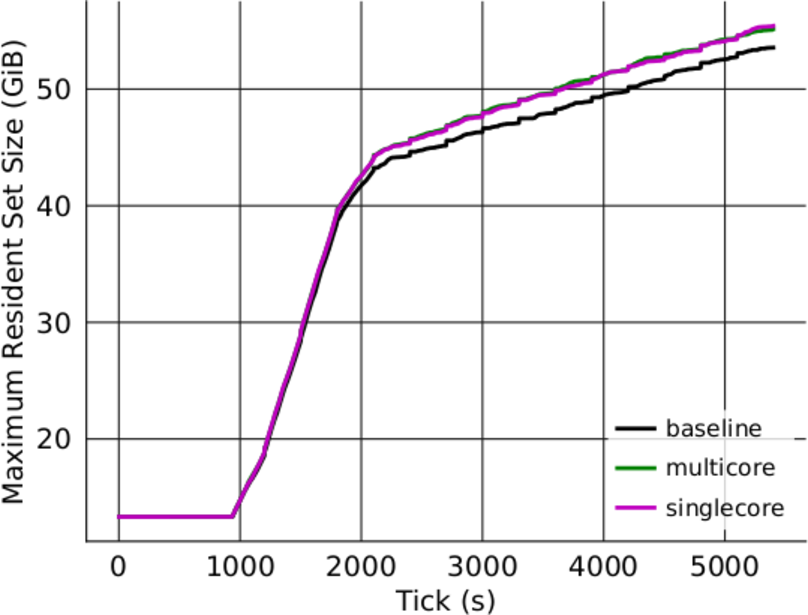
\includegraphics[clip, width=1.0\textwidth]{images/overhead_memory.pdf}
		\caption{Simulation Memory}
		\label{fig:overhead_shadow}
	\end{subfigure}
	\caption{Global Overhead --- Comparison of overhead in pure multicore
          and singlecore network %% conditions.
          Figure~\ref{fig:overhead_ttlastbyte} shows two sets of %% download
          time CDF curves for each file size (2 MiB and 5 MiB), %%
          Figure~\ref{fig:overhead_throughput} shoes the 5 minute moving average
          %% throughput over time, and Figure~\ref{fig:overhead_shadow} shows
          the %% memory consumption across the experiment lifetime. The
          simulation %% includes 100 relays, 2 authorities, 1 ledger authority,
          10 %% intermediaries and 1000 Tor clients scaled down from the public
          consensus file `2018-02-03-00-00-00-consensus'.}
	\label{fig:overhead}
\end{figure*}

A substantial contribution of the research is embedded within our implementation
of the moneTor framework. The modifications, applied to Tor release version
0.3.2.10, cover approximately fifteen thousand added lines of code across Tor's
core C software. We emphasize that the implementation is engineered solely for
our experiments. Most notably, expensive cryptographic operations such as ZKPs
and commitments were simulated using methods that account for Shadow's unique
virtual time management~\cite{jansen2011shadow}. We consider both scenarios in
which the simulated Tor process is running on a multicore or singlecore
processor. In the multicore case, the cryptographic operations are replaced by
an ``idle'' command that allows the virtual node to complete other tasks in
parallel. In the singlecore case, cryptographic operations are simulated by
looping through a series of dummy SHA256 Hash operations.
%Since Shadow intercepts these AES
%calls and in turn replaces them with virtual CPU delays, we can optimize
%real-life run time while allowing Shadow to accurately account for the virtual
%computation. 
Using these methods, duration of the delays were tuned to conservatively reflect
real measurements in prior background
work~\cite{green2017bolt}.\footnote{Extracted values are conservative in the
  sense that our zero-knowledge proofs require proving only a subset of the
  statements required in each corresponding Bolt zero-knowledge proof.} Note
that our prototype does not implement anything that does not help us to answer
our research goals, such as coin/wallet management, extension of the Tor control
protocol to manage the asset and various options, Intermediary information
recovery in case of crash, etc. The prototype serves the following purposes in
our study.
\begin{enumerate}
\item An implementation covering nuances not explicitly covered in the protocol
  designs. In effect, we would like to show that there are no unexpected and
  prohibitive practical conflicts with the existing Tor design.
\item A platform to study the feasibility of premium circuit prioritization from
  a networking perspective.
\item A platform to obtain a rough factor-of-two approximation for all
  bandwidth, computation, and memory requirements of the system, both globally
  and at individual nodes.
\end{enumerate}

The first design purpose is clearly qualitative and we briefly note that we did
not discover any insurmountable logical flaws in the design. To analyze the
networking dynamics and resource consumption, we studied our implementations
through the following experiments.

\subsection{Methodology}
\label{subsec:methodology}


Experiments were conducted using the Tor shadow simulator
tool~\cite{jansen2011shadow, tracey2018high}. We ran two sets of experiments at
different scales from a consensus document published in early February 2018. The
first set featured 100 relays, 1000 clients, 10 intermediaries, and ran for a
total of 90 minutes. These experiments were used to gather information
concerning the system overhead and protocol execution times. The second set
featured 250 relays, 2500 clients, 25 intermediaries, 80 minutes of total run
time, and was used to measure the performance benefits conferred to premium
clients. In both cases, simulated traffic features 8\% \emph{bulk} clients who
continuously download 5 MiB files and 92\% \emph{web} clients who periodically
download 2 MiB files~\footnote{While 5 MiB bulk files are a common standard in
  Tor benchmarking~\cite{portal2018tormetrics}, 2 MiB web files reflect the
  approximate size of modern web pages~\cite{team2018httparchive}}. The number
and behavior of clients were chosen to satisfy (A) realistic congestion rates
measured by a transfer timeout percentage around 4\%~\cite{portal2018tormetrics}
and a historical bulk/web global traffic ratio of about
25\%/75\%~\cite{privcount-ccs2016, learning-ccs2018}. Importantly, it should be
noted that neither the scale of our experiments nor the precise configuration of
client nodes are intended to be precise replicas of real-world conditions. Tor
networking is itself a complex area of research and we are content to adopt the
simplest model that will highlight the relatively crude networking needs of our
incentivization scheme.

\subsection{Experiments}
\label{subsec:experiments}
Our experiments are separated into three groups each capturing a separate
characteristic of the scheme.

\paragraph*{Global Overhead}
First, we attempt to show the total cost of the moneTor scheme in terms of total
network throughput. To highlight worst-case performance, we configured a medium
scale experiment consisting of 100\% of premium clients and compare to a
baseline trial with 0\% premium clients. The payment protocols run but the
control-flow and EWMA stay unchanged to only compare the CPU cost of the payment
scheme (that is, we do not apply any priority function). Since our algorithms
makes use of some concurrent crytpographic operations, we are concerned with the
number of CPU cores available to most relays. This information is not publicly
available. As a result, we provide two trials with moneTor: one where we assume
all nodes are running on multi-core hardware and one in which all nodes are
running on single-core hardware. The results are summarized in
Figure~\ref{fig:overhead}.

% Add information about how we simulate singlecore and multicore hardware
% That gonna overflow 12 pages, though :/

\begin{figure*}[t] \centering
	\begin{subfigure}[t]{0.32\textwidth} \centering
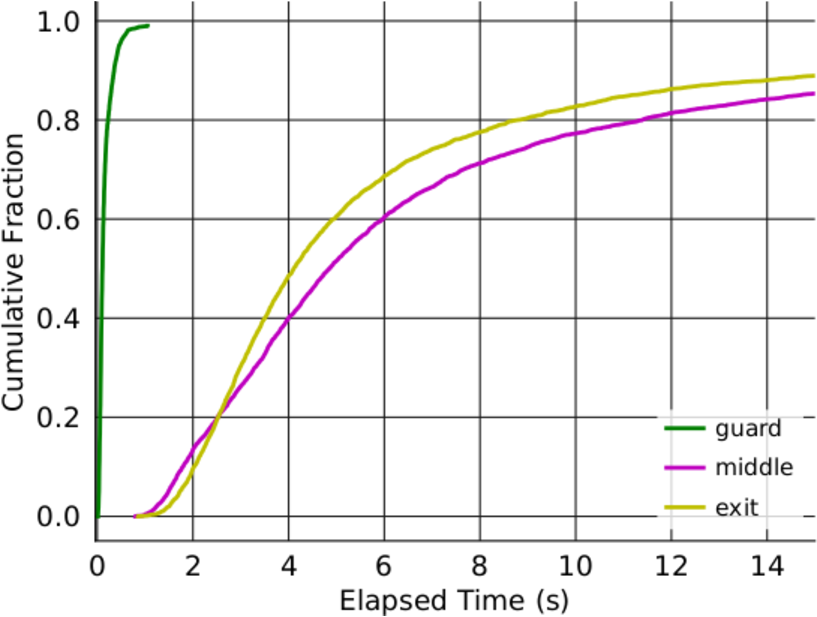
\includegraphics[trim={0 0cm 0 0cm}, clip,
  width=1.0\textwidth]{images/payment_establish.pdf}
		\caption{Nano-Establish - Built after the circuit construction,
                  but before the circuit usage!}
\label{fig:payments_establish}
	\end{subfigure}
	\begin{subfigure}[t]{0.32\textwidth} \centering
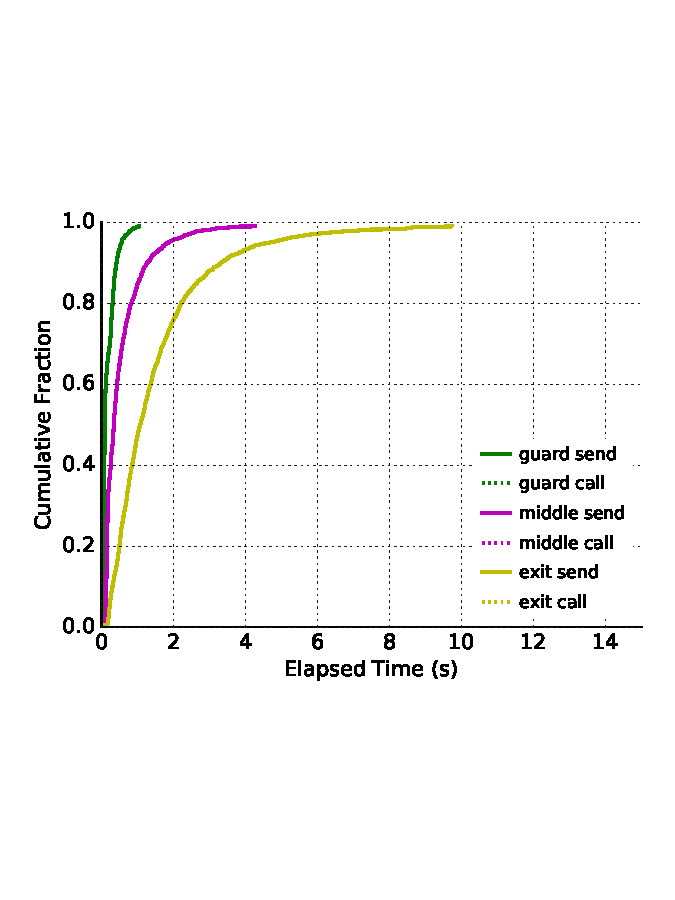
\includegraphics[trim={0 0cm 0 0cm}, clip,
  width=1.0\textwidth]{images/payment_pay.pdf}
		\caption{First Payment - Should match 1 half RTT if the
                  preemptive Nano-Establish is perfect}
\label{fig:ttfp}
	\end{subfigure}
	\begin{subfigure}[t]{0.32\textwidth} \centering
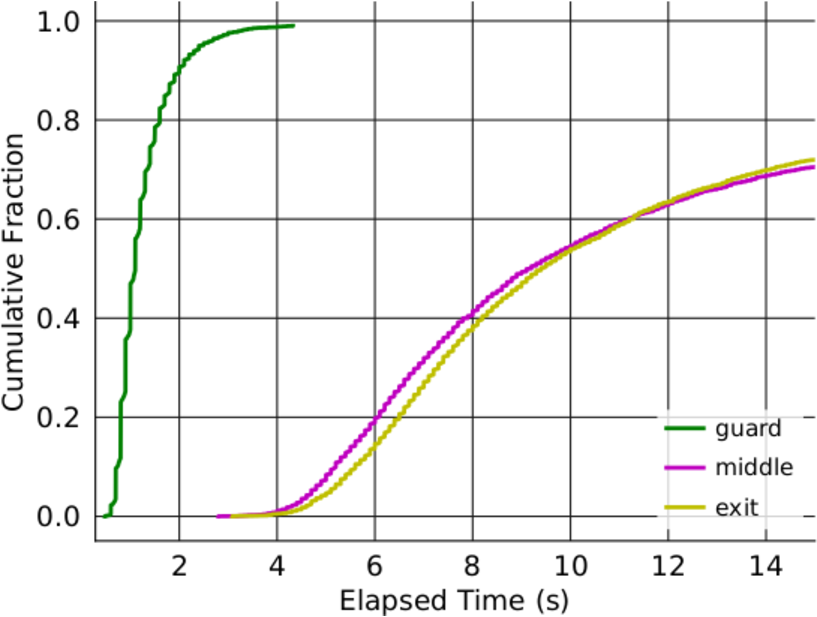
\includegraphics[trim={0 0cm 0 0cm}, clip,
  width=1.0\textwidth]{images/payment_close.pdf}
		\caption{Nano-Close - Happens just before the circuit is
                  destroyed}
\label{fig:payments_close}
	\end{subfigure}
	\caption{Protocol Execution Time --- Time to finish each protocol step
          split across interactions with each of the three relays. The
          simulation includes 100 relays, 2 authorities, 1 ledger authority, 10
          intermediaries and 1000 Tor clients scaled down from the public
          consensus file `2018-02-03-00-00-00-consensus'.}
\label{fig:latencymeasurements}
\end{figure*}

Our findings indicate that even in the worst case scenario, our system incurs
statistically negligible overhead at these scales across the two measures of
download time (e.g., less than 2\% increase on the mean web download for the
singlecore experiment), throughput, and memory usage. This in line with the raw
bandwidth observations in which a small fraction ($< 1\%$) of the network
traffic is attributable to moneTor payment messages. This is true for all of our
trials which feature a payment rate of 1 payment (1 cell) every 1000 data cells
exchanged in either direction. It is also possible to increase the payment rate
for more fairness if needed, as long as the total overhead induced from control
cells is kept under an acceptable fraction of the overall data bandwidth.
%%%
% Reading this sentence appears to be unclear to me
%%%
%This
%low overhead cost is separate from adverse networking effects of prioritization,
%which has the potential to more drastically affect performance.

%\begin{table}
%  \caption[Overhead Throughput Total]{\textbf{Overhead Throughput Total} Total
%    transferred application traffic over the duration of the over head trials
%    compared to total transferred payment traffic.}
%  \begin{center}
%    \begin{tabular}{ c c c }
%      & Throughput (GiB) & Payment Traffic (GiB) \\ \hline
%      Baseline & 128.4 & 0.000 \\
%      Multi-Core & 129.1 & 0.449 \\
%      Single-Core & 127.6 & 0.396
%    \end{tabular}
%  \end{center}
%  \label{tab:overhead}
%\end{table}


\paragraph*{Payment Latency}
Given results from our data collection, we surmise that payment latency is a
crucial factor in servicing our front-loaded clients. To this end, we measure
the distribution of completion times for various steps in the protocol. To
highlight the effects of native latency in the Tor network, we show payments
split across each relay role of guard, middle, and exit. Recall that moneTor
makes use of high-overhead, low-marginal cost payment channels (i.e., the
channels take time to build but the client needs them long after they are
built). The bulk of the cost in our scheme lies in the conduction of the
nanopayment channel \emph{establish} and \emph{close} protocols as shown in
Figure~\ref{fig:payments_establish} and Figure~\ref{fig:payments_close}. Notice
that close operations are about twice as time consuming as establish operations
reflecting the need for the relay to close his half of the nanopayment channel
before the client can complete hers. Figure~\ref{fig:ttfp} illustrates time to
first payment, our most revealing latency metric. This measure includes the
overhead in channel establishment when we do not have available preemptive
channels. In the best case scenario, when all three payment channels have been
correctly pre-built for the circuit, this measure is equivalent to a single trip
toward each relay. Comparing this Figure~\ref{fig:ttfp} to
Figure~\ref{fig:payments_establish}, we observe the effectiveness of preemptive
channel building. The other observation sustaining the effectiveness of the
pre-built strategy is the recorded time for the ``call'' versus ``send'': if no
delay is observed, the pre-built was a success.

In all protocol phases, we observe that latency for guard relays are negligible
in comparison to the middle and exit relays, further validating our design
decision to implement special directly paid guard channels (that is, since a
guard is not expected to see all Tor clients in the entry position, it may
allocate itself micropayment channels for the subset of clients it serves).

\paragraph*{Network Priority}
\label{sec:priority_exp}
Our final set of experiments studies the success of our scheme in delivering
prioritized traffic for premium users. To perform this analysis, we prepared
sets of three small experiments with varying modifier priorities $\alpha \in
\{0, 0.25, 0.5\}$ and $\beta \in \{1, 5, 10\}$, where $\alpha = 0, \beta = 1$
represents vanilla Tor when payments are off. In our set of experiments, we
assume 25\% of premium users. From Figures \ref{fig:modifier_pr25_web},
\ref{fig:modifier_pr25_bulk}, and \ref{fig:modifier_pr25_all}, we observe
interesting information. First, variations in our network-wide tunable
parameters do offer differentiation in download speed. Yet, as we detail in
appendix~\ref{sec:scheduling}, offering bandwidth differentiation for the Tor
network is more complex than previously exposed. Indeed, the current state of
the Tor network (congestion in the exit interface) makes local scheduling
priority ineffective for most circuits, while this method worked fine with
previous work when the Tor network was in a very different shape. Second, the
differentiation in bandwidth for $\alpha = .25, \beta=5$ ``averages out'' to
approximately mirror the baseline experiment, indicating little loss in overall
network performance, and confirming our overhead experiment (recall 25\% of
premium users). Nevertheless, our result for $\alpha = 0.5, \beta=10$ indicates
that the performance degrades faster for nonpremium the closer we are to the
maximum gain we could obtain for the premium users. This result also highlight
the complexity within the choice of the right set of parameters or techniques to
offer efficient prioritization which, since a poor choice of parameters can lead
to an overall decrease of throughput. One of the take-out message of our
research and results, is that we believe the prioritization scheme to be more
complex to get right and fulfill its goal in practice than the design of the
anonymous payment layer itself.

%Note, one difference of the edge window-based priority mechanism over a scheduling 
%approach is
%that the latency is unchanged: there is no reason for the first byte to come
%faster for premium users since our priority mechanism only changes the size of
%the control flow window (i.e., how many cells the circuit is allowed to carry at
%any time. See Section~\ref{subsub:prioritized} for details). Such an approach
%keeps the network responsive for nonpremium and low-bandwidth usage, while still
%offering an upward benefit for premium users loading standard-to-large web pages, as 
%shown in Figure~\ref{fig:modifier}.

Note that our analysis of the scheme holds the total network capacity static.
However Tor incentives build on the premise that everybody would benefit from
new relays added in new locations. We believe that in the worst-case scenario
from a performance viewpoint, we would obtain similar performance than the
static analysis since it might be possible that Tor usage grows proportionally
to the added relays. That is the main reason why we did not experiment with
simulated added capacity: globally better performance for everyone could be
misleading.
%However, even in such case, all users would benefit from better anonymity from the new distribution of relays. Moreover, advancing human rights and freedoms to more people would be achieved, which outweighs performance benefit from any simulated static user base with higher Tor network capacity experiment. 


\begin{figure*} \centering
	%\begin{subfigure}[t]{0.32\textwidth} \centering
%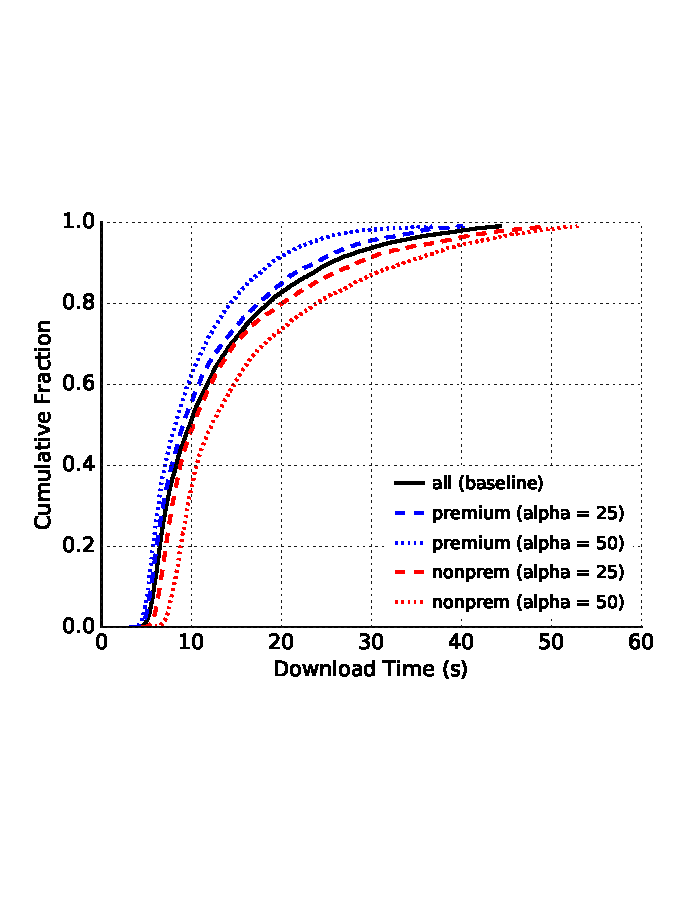
\includegraphics[trim={0 3cm 0 3cm}, clip, width=1.0\textwidth]{images/modifier_pr50_web.pdf}
		%\caption{Web Download Time}
%\label{fig:modifier_pr50_web}
	%\end{subfigure} \begin{subfigure}[t]{0.32\textwidth} \centering
%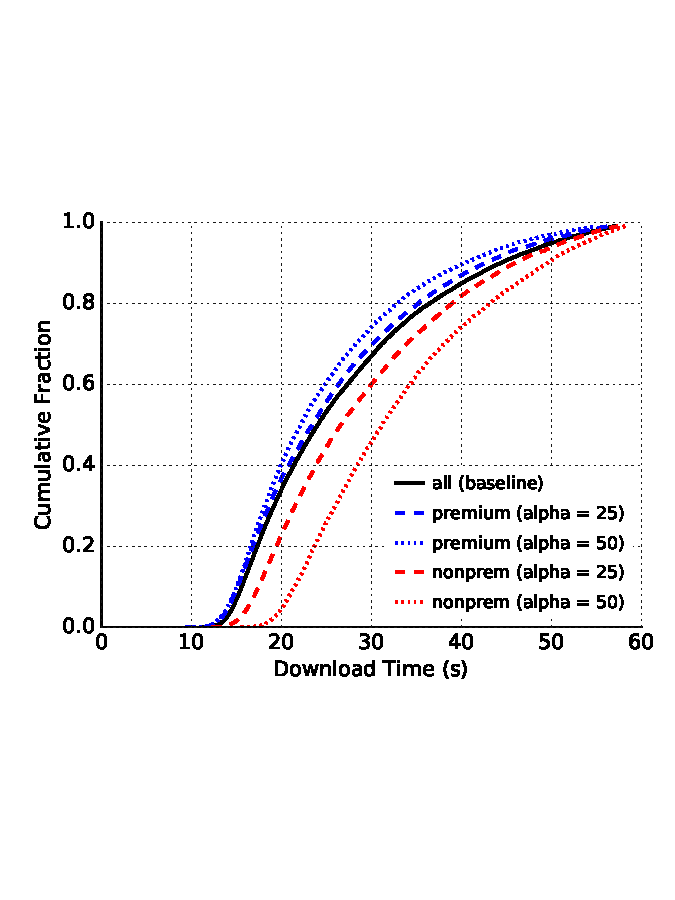
\includegraphics[trim={0 3cm 0 3cm}, clip, width=1.0\textwidth]{images/modifier_pr50_bulk.pdf}
		%\caption{Bulk Download Time}
%\label{fig:modifier_pr50_bulk}
	%\end{subfigure} \begin{subfigure}[t]{0.32\textwidth} \centering
%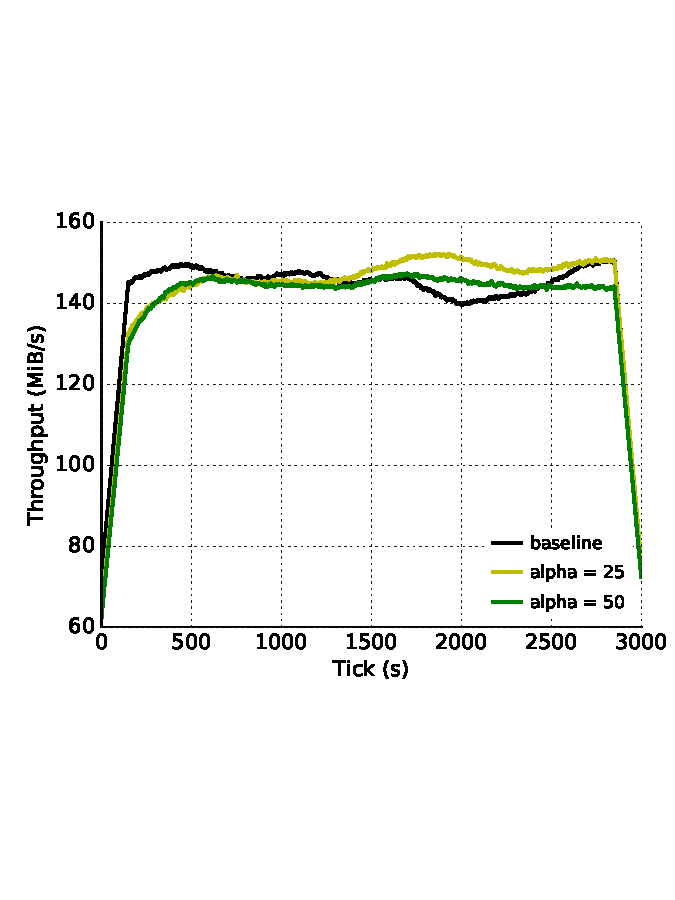
\includegraphics[trim={0 3cm 0 3cm}, clip, width=1.0\textwidth]{images/modifier_pr50_all.pdf}
		%\caption{Throughput}
%\label{fig:modifier_pr50_all}
	%\end{subfigure}
	\begin{subfigure}[t]{0.32\textwidth} \centering
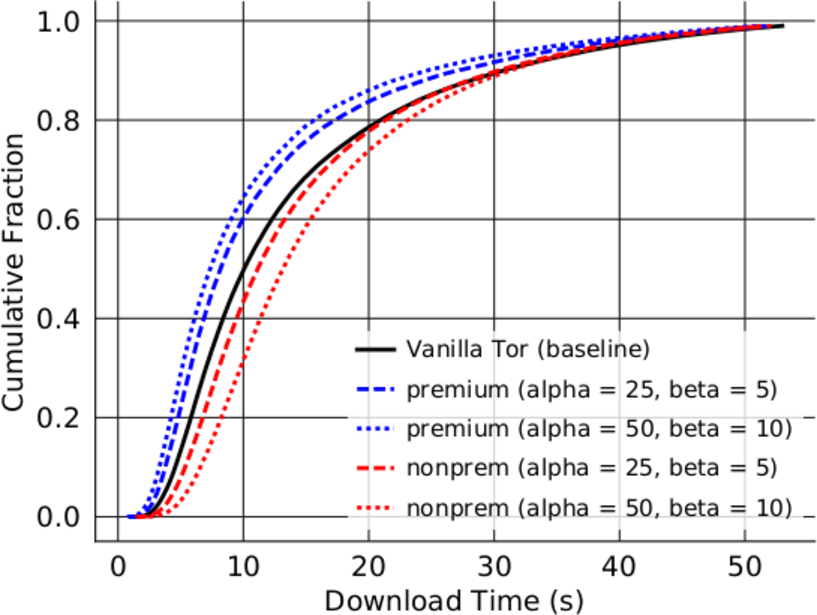
\includegraphics[trim={0 0cm 0 0cm},
  clip,width=1.0\textwidth]{images/modifier_pr25_web_lowloss.pdf}
		\caption{Web Download Time}
\label{fig:modifier_pr25_web}
	\end{subfigure}
	\begin{subfigure}[t]{0.32\textwidth} \centering
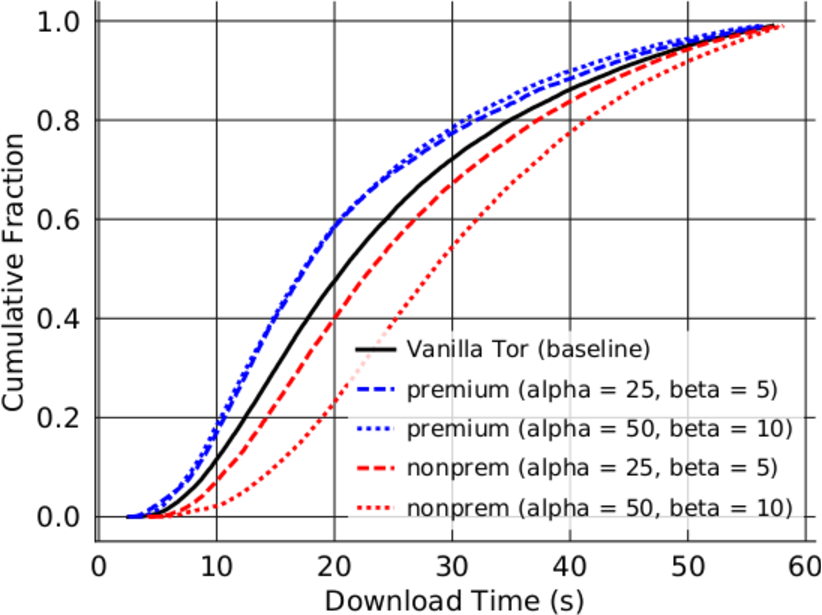
\includegraphics[trim={0 0cm 0 0cm}, clip,
  width=1.0\textwidth]{images/modifier_pr25_bulk_lowloss.pdf}
		\caption{Bulk Download Time}
\label{fig:modifier_pr25_bulk}
	\end{subfigure}
	\begin{subfigure}[t]{0.32\textwidth} \centering
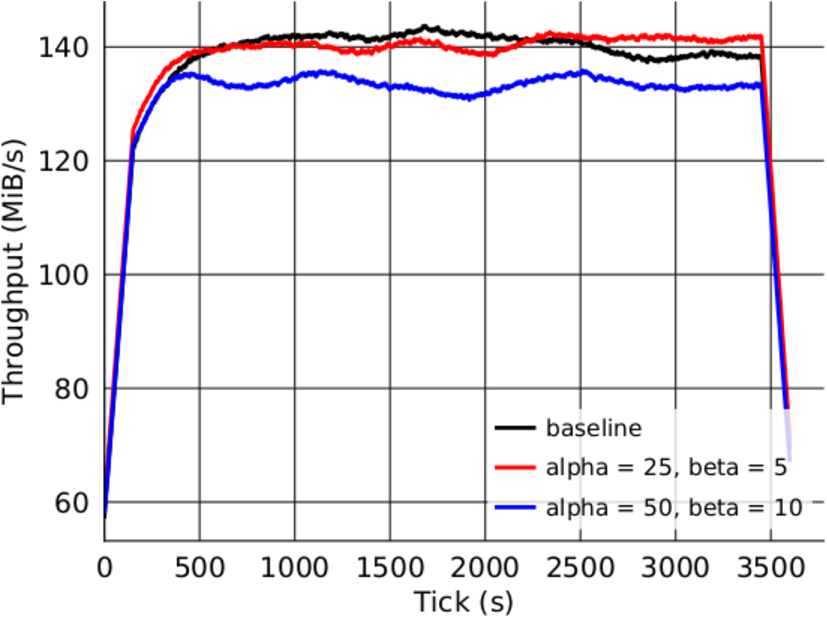
\includegraphics[trim={0 0cm 0 0cm}, clip,
  width=1.0\textwidth]{images/modifier_pr25_all_lowloss.pdf}
		\caption{Total throughput, all clients}
\label{fig:modifier_pr25_all}
	\end{subfigure}
	\caption{Prioritization Benefit --- Performance differentiation between
          paid and unpaid users. We display results for 25\% premium users.
          Simulations feature 250 relays, 2 authorities, 1 ledger authority, 25
          intermediaries and 2500 Tor clients scaled down from the public
          consensus file `2018-02-03-00-00-00-consensus'.}
\label{fig:modifier}
\end{figure*}

%\begin{table}
%  \caption[Prioritized Throughput]{\textbf{Prioritized Throughput} Tabulate total
%    number of successful file transfers and timeout errors across varying levels
%    of prioritization}
%  \begin{center}
%    \begin{tabular}{ c c c c}
%      & Throughput & Timeouts & Timeout \\
%      & (GiB) & (Web) & (Bulk) \\ \hline
%      $\alpha = 0.00$ & 427 & 115 & 354 \\ \hline
%      $\alpha = 0.25,\ pr\% = 50$ & 429 & 206 & 404 \\
%      $\alpha = 0.25,\ pr\% = 25$ & 433 & 231 & 459 \\ \hline
%      $\alpha = 0.50,\ pr\% = 50$ & 420 & 233 & 356 \\
%      $\alpha = 0.50,\ pr\% = 25$ & 414 & 381 & 513 \\
%    \end{tabular}
%  \end{center}
%  \label{tab:modifier}
%\end{table}

%%% Local Variables:
%%% mode: latex
%%% TeX-master: "../main"
%%% End:
